% Chapter 4 from the standard thesis template
% that contains an adv. example table and figure.
\chapter{SOFTWARE DEFINED RADIO BASED RADIOMETER IMPLEMENTATION}\label{ch:implementation}

This chapter examines the implementation of a software defined radio based radiometer.  First we will examine requirements of both a traditional radiometer and a Software Defined Radio (SDR) based radiometer.  Next we will map the traditional radiometer components discussed in chapter \ref{ch:background} to their digital counterparts.  Finally a high level overview of the operation of a SDR-based radiometer and what impact that has on the performance of the radiometer.

\section{Requirements}\label{requirements}

This section discusses the hardware and software requirements used to drive the selection of the hardware and software platforms use to implement our software defined radio based radiometer.  

\emph{Hardware Requirements.}  The capabilities of existing traditional radiometers were the primary driving force in setting the requirements of our hardware development platform.  Dr. Brian Hornbuckle from the Electrical and Computer Engineering and Agronomy department at Iowa State University was consulted with respect to key specifications of his radiometer.  Additionally, the specifications of other radiometers were examined. 

Table \ref{rad_performance} summarizes the specification of three parameters that were decided upon for selecting our hardware development platform, based on our investigation.  This lead to the selection of the N200 software defined radio platform with a DBSRX2 daughter board from Ettus Research as our hardware platform.  Section \ref{SDR_platform} provides more in depth information on the hardware used and why it was selected.

\begin{table}[h!tb] \centering
\isucaption{Required Radiometer performance}
\label{rad_performance}
% Use: \begin{tabular{|lcc|} to put table in a box
\begin{tabular}{lcc} \hline
\textbf{Parameter} & \textbf{Value} & \textbf{Units} \\ \hline
Minimum bandwidth & 20 & MHz \\
Operational frequency & 1400 - 1420 & MHz \\
$NE\Delta T$ (sensitivity) & 1 & Kelvin \\ \hline
\end{tabular}
\end{table}

\emph{Software Requirements.}  Since an objective of this work was to help make radiometers more wildly accessible to the general research and education community, a requirement of the development software was ease of use.  Additionally, the user interfaces developed with these software tools needed to be easy to use, while providing sufficient computing efficiency for the signal processing required for radiometry.

GNURadio met the stated requirements.  It includes a supplemental software package called GNURadio Companion (GRC), which uses a graphical interface for creating a radio environment.  GNURadio and GRC are discussed in greater detail in Section \ref{software_platform}.

\section{Mapping Traditional Radiometer Functions to a Software Defined Radio Based Radiometer}

The use of a software defined radio (SDR) to implement a radiometer requires mapping components of a traditional radiometer to SDR-based technology.  This section presents the mapping of three such components for implementing our SDR-based radiometer.  These components are:  1) power measurement, 2) data smoothing, and 3) bandwidth limiting and filtering.

\subsection{Power measurement}

A traditional radiometer uses a device called a square law detector to measure power.  This device is a diode that operates in the square law region.  While the diode is operating in this region, the output voltage ($V_{out}$)is proportional to the square of the input voltage ($V_{in}$) and is therefore proportional to the input power ($P_{in}$).  This relationship is shown in Equation \ref{square_eq} [\cite{Navy_detector}].  Figure \ref{square_law_simple} shows a simple circuit diagram and input and output voltages from this circuit.

\begin{equation}\label{square_eq}
V_{out} = nV_{in}^2 = nP_{in}
\end{equation}

{\begin{figure}[h!tb] 
\centering
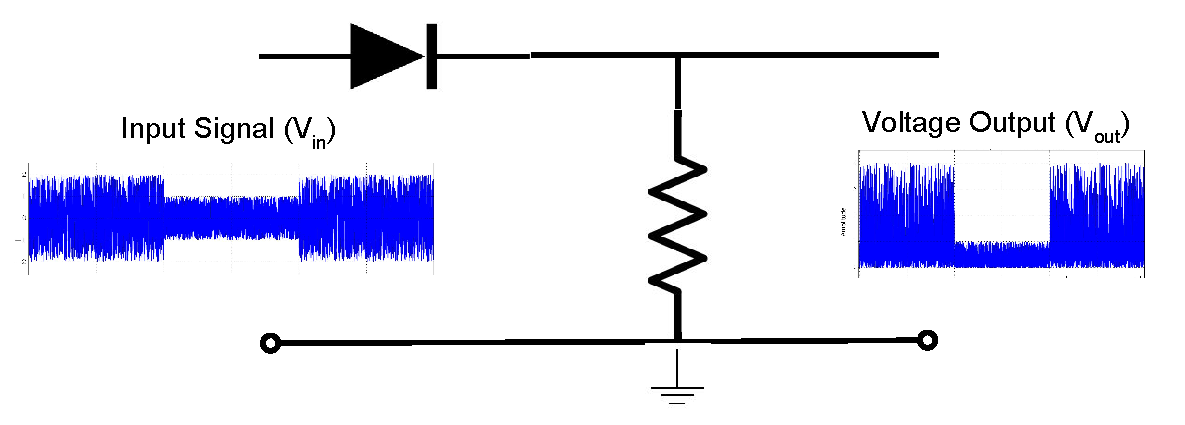
\includegraphics[width=17cm]{Images/square_law.pdf}
\isucaption{A simple diagram of a square-law detector.}
\label{square_law_simple}
\end{figure}
}

The software defined radio based radiometer operates in a similar manner as a traditional radiometer.  With the SDR-based radiometer our signal is converted to I (in-phase) and Q (quadrature-phase).  Adding the I and Q data allows us to recreate the signal.  The I and Q data contains the magnitude of the in-phase and quadrature-phase information respectively.  When summed this represents the magnitude of the original signal.  To determine the total power, the magnitude is squared to produce an output that represents the total power of the signal ($P_{out}$).  Equation \ref{sdr_x2} gives the mathematical representation of a software defined radio based radiometer implementation of a square law detector[\cite{Rashid}]. 

\begin{equation}\label{sdr_x2}
I^2+Q^2 = P_{out}
\end{equation}

Figure \ref{square_block} shows the block within GNURadio Companion that performs the function of total power measurement.  In Figure \ref{square_block}, the block labeled as A performs mathematically the power detection as shown in Equation \ref{sdr_x2}.  Block C decimates the data to reduce the sample size and thus reduce the file size of the data.  

{\begin{figure}[h!tb] 
\centering
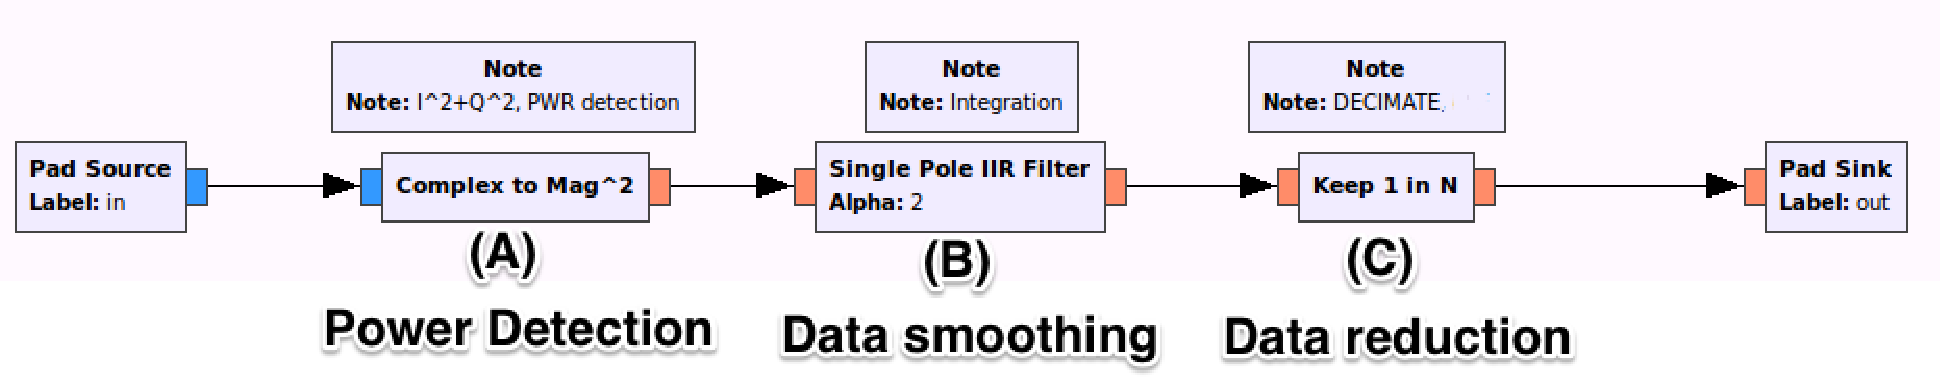
\includegraphics[width=17cm]{Images/TPR_grc.png}
\isucaption{A block diagram of the power detection, low pass filter and decimation block used for total power measurements.}
\label{square_block}
\end{figure}
}

For both a traditional radiometer and a SDR-based radiometer, the output of this total power information will fluctuate rapidly.  To smooth this signal we send this signal through a low pass filter which is shown in Figure \ref{square_block} as block B.  This smoothing will be discussed in the next section.

\subsection{Data smoothing}\label{smoothing}

Output from the power detection system is noisy, which makes detecting small changes in power difficult (i.e. hinders sensitivity).  Figure \ref{square_raw} shows an example of this noisy output from a square-law detector.

{\begin{figure}[h!tb] 
\centering
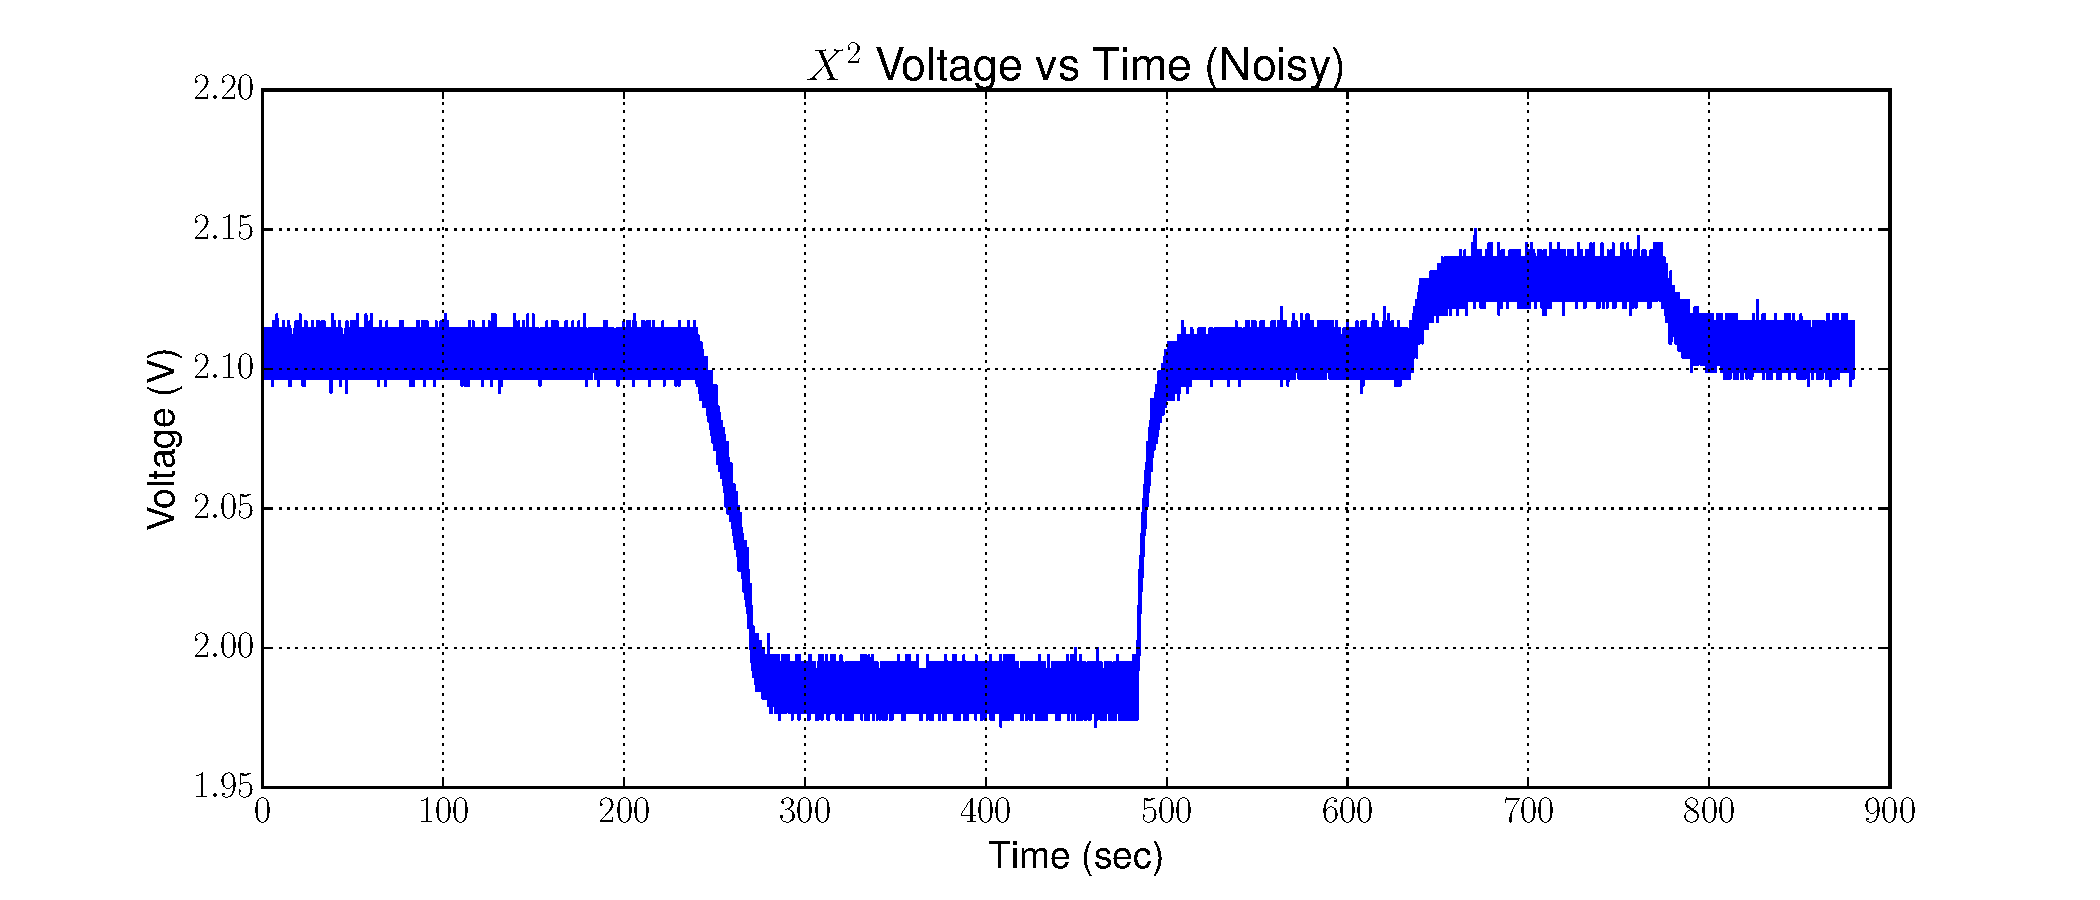
\includegraphics[width=17cm]{Experiments/Exp1/noisy_voltage.pdf}
\isucaption{Power measurements from a square law detector before filtering}
\label{square_raw}
\end{figure}
}

A traditional radiometer will use an integrator, which is equivalent to a low pass filter, to smooth the output from the square-law detector.  This low pass filter is implemented as a simple RC circuit as shown in Figure \ref{rc_circuit}.  This low pass filter allows us to reduce the noise and this results in Figure \ref{square_raw_filt}.  

{\begin{figure}[h!tb] 
\centering
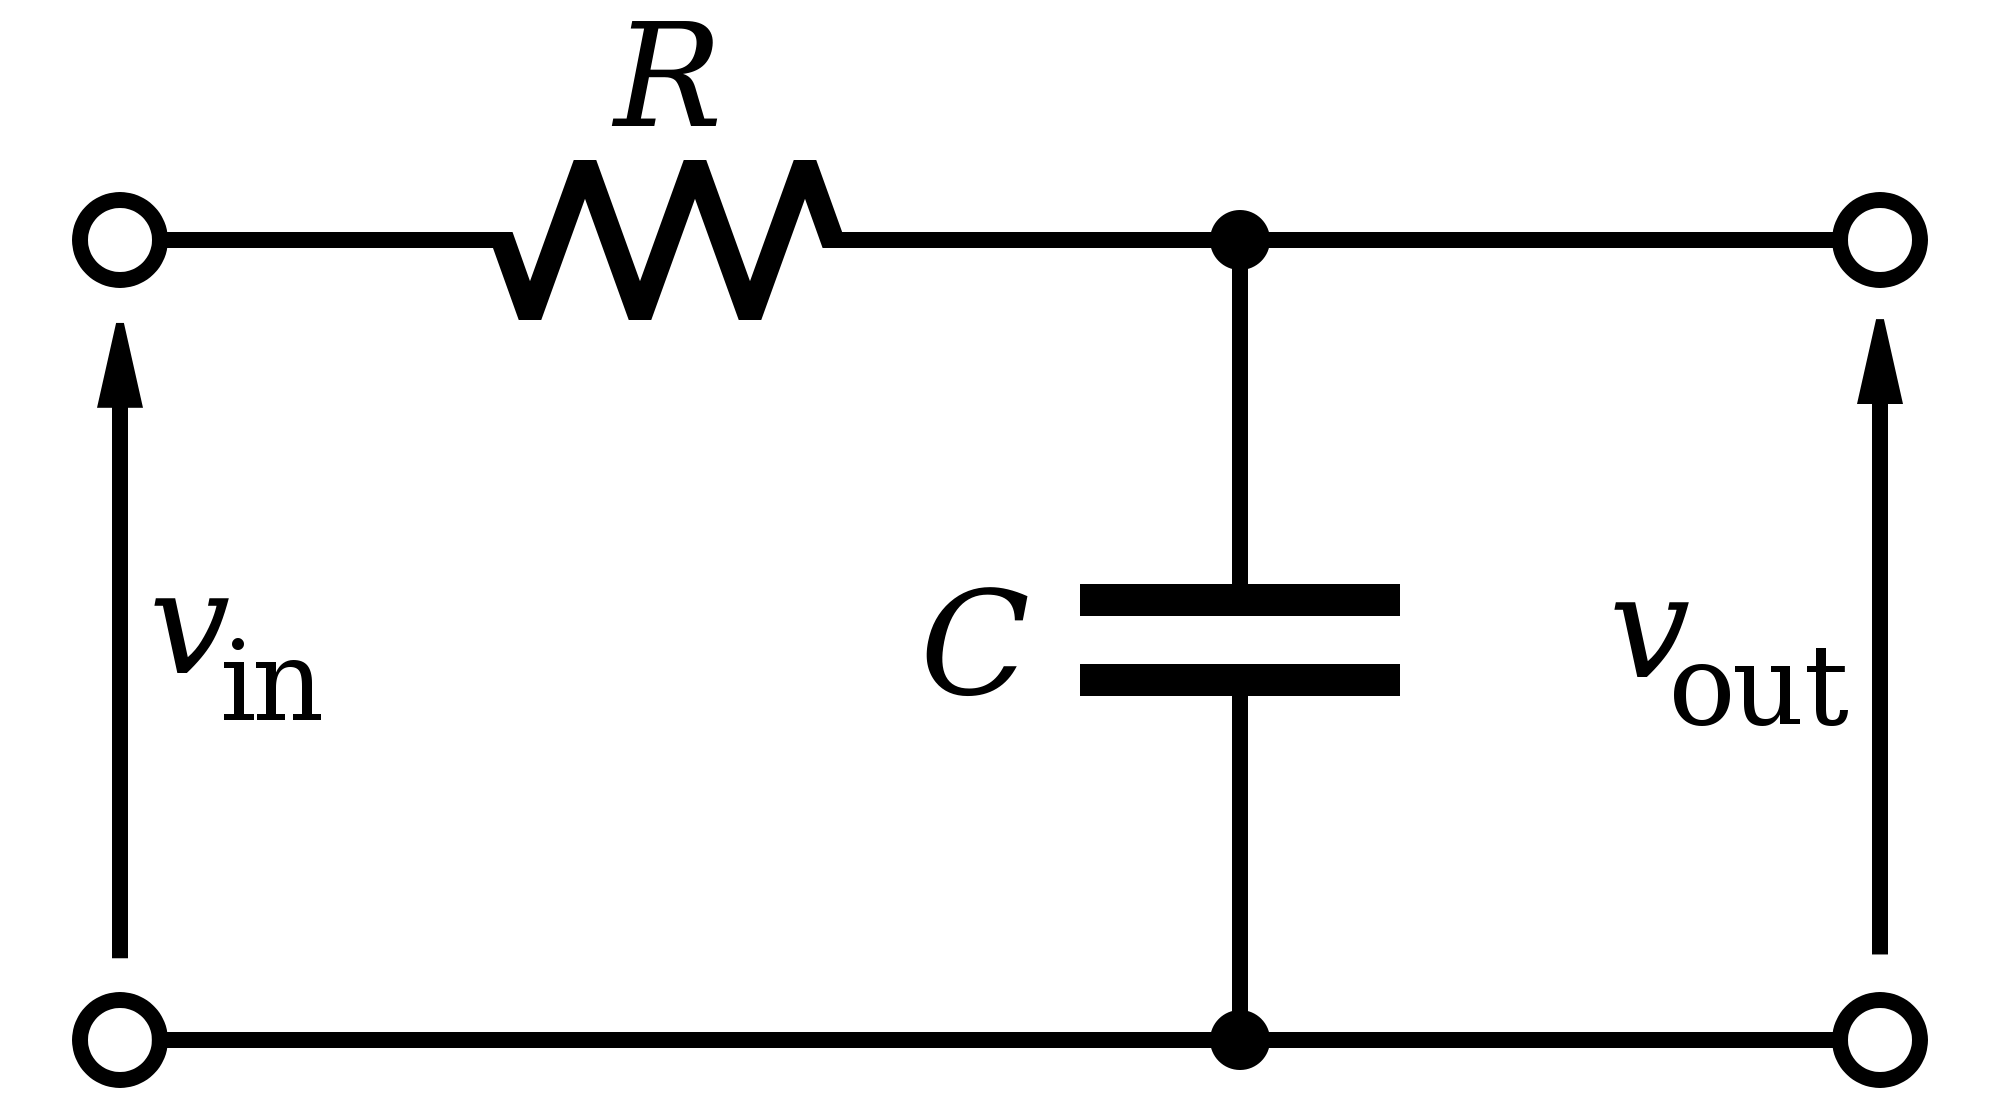
\includegraphics[width=6cm]{Images/rc_lpf.png}
\isucaption{A simple RC circuit.}
\label{rc_circuit}
\end{figure}
}

{\begin{figure}[h!tb] 
\centering
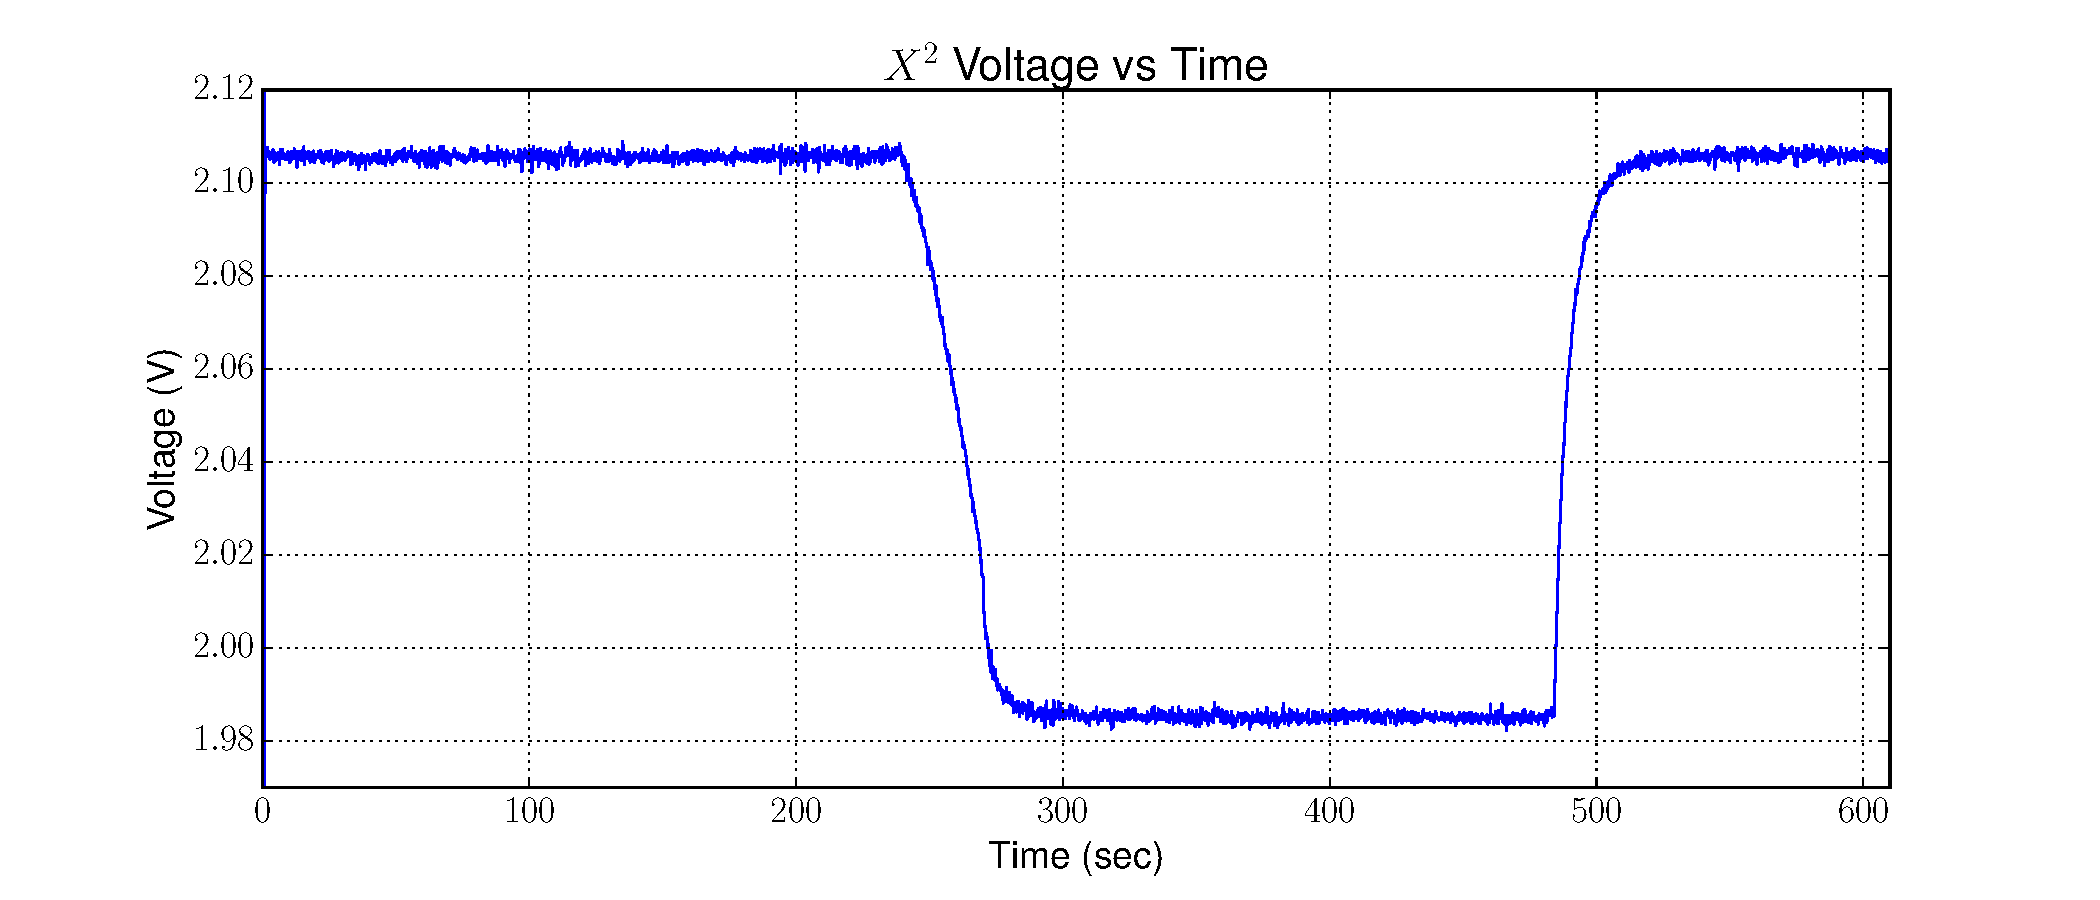
\includegraphics[width=17cm]{Experiments/Exp1/x2_filter.pdf}
\isucaption{Power measurements from a square law detector after filtering}
\label{square_raw_filt}
\end{figure}
}

%This RC filter is described by the Laplace transform of its impulse response.  This RC filter is shown in Equation \ref{RC_laplace} where $K$ is the gain of the filter, $\tau$ is the time constant of the filter and $s$ is the Laplace transform variable.

%\begin{equation}\label{RC_laplace}
%\frac{Output}{•Input} = K \frac{1}{\tau s + 1}
%\end{equation}

We can now look at the step response of this filter as shown in Figure \ref{rc_response} in the top left and top right graph.  To implement this low pass filter as a digital filter, a single pole Infinite Impulse Response (IIR) filter is used.  We can examine how a IIR filter is identical to a RC filter by looking at the step response of this filter as we did with the RC filter step response.

{\begin{figure}[h!tb] 
\centering
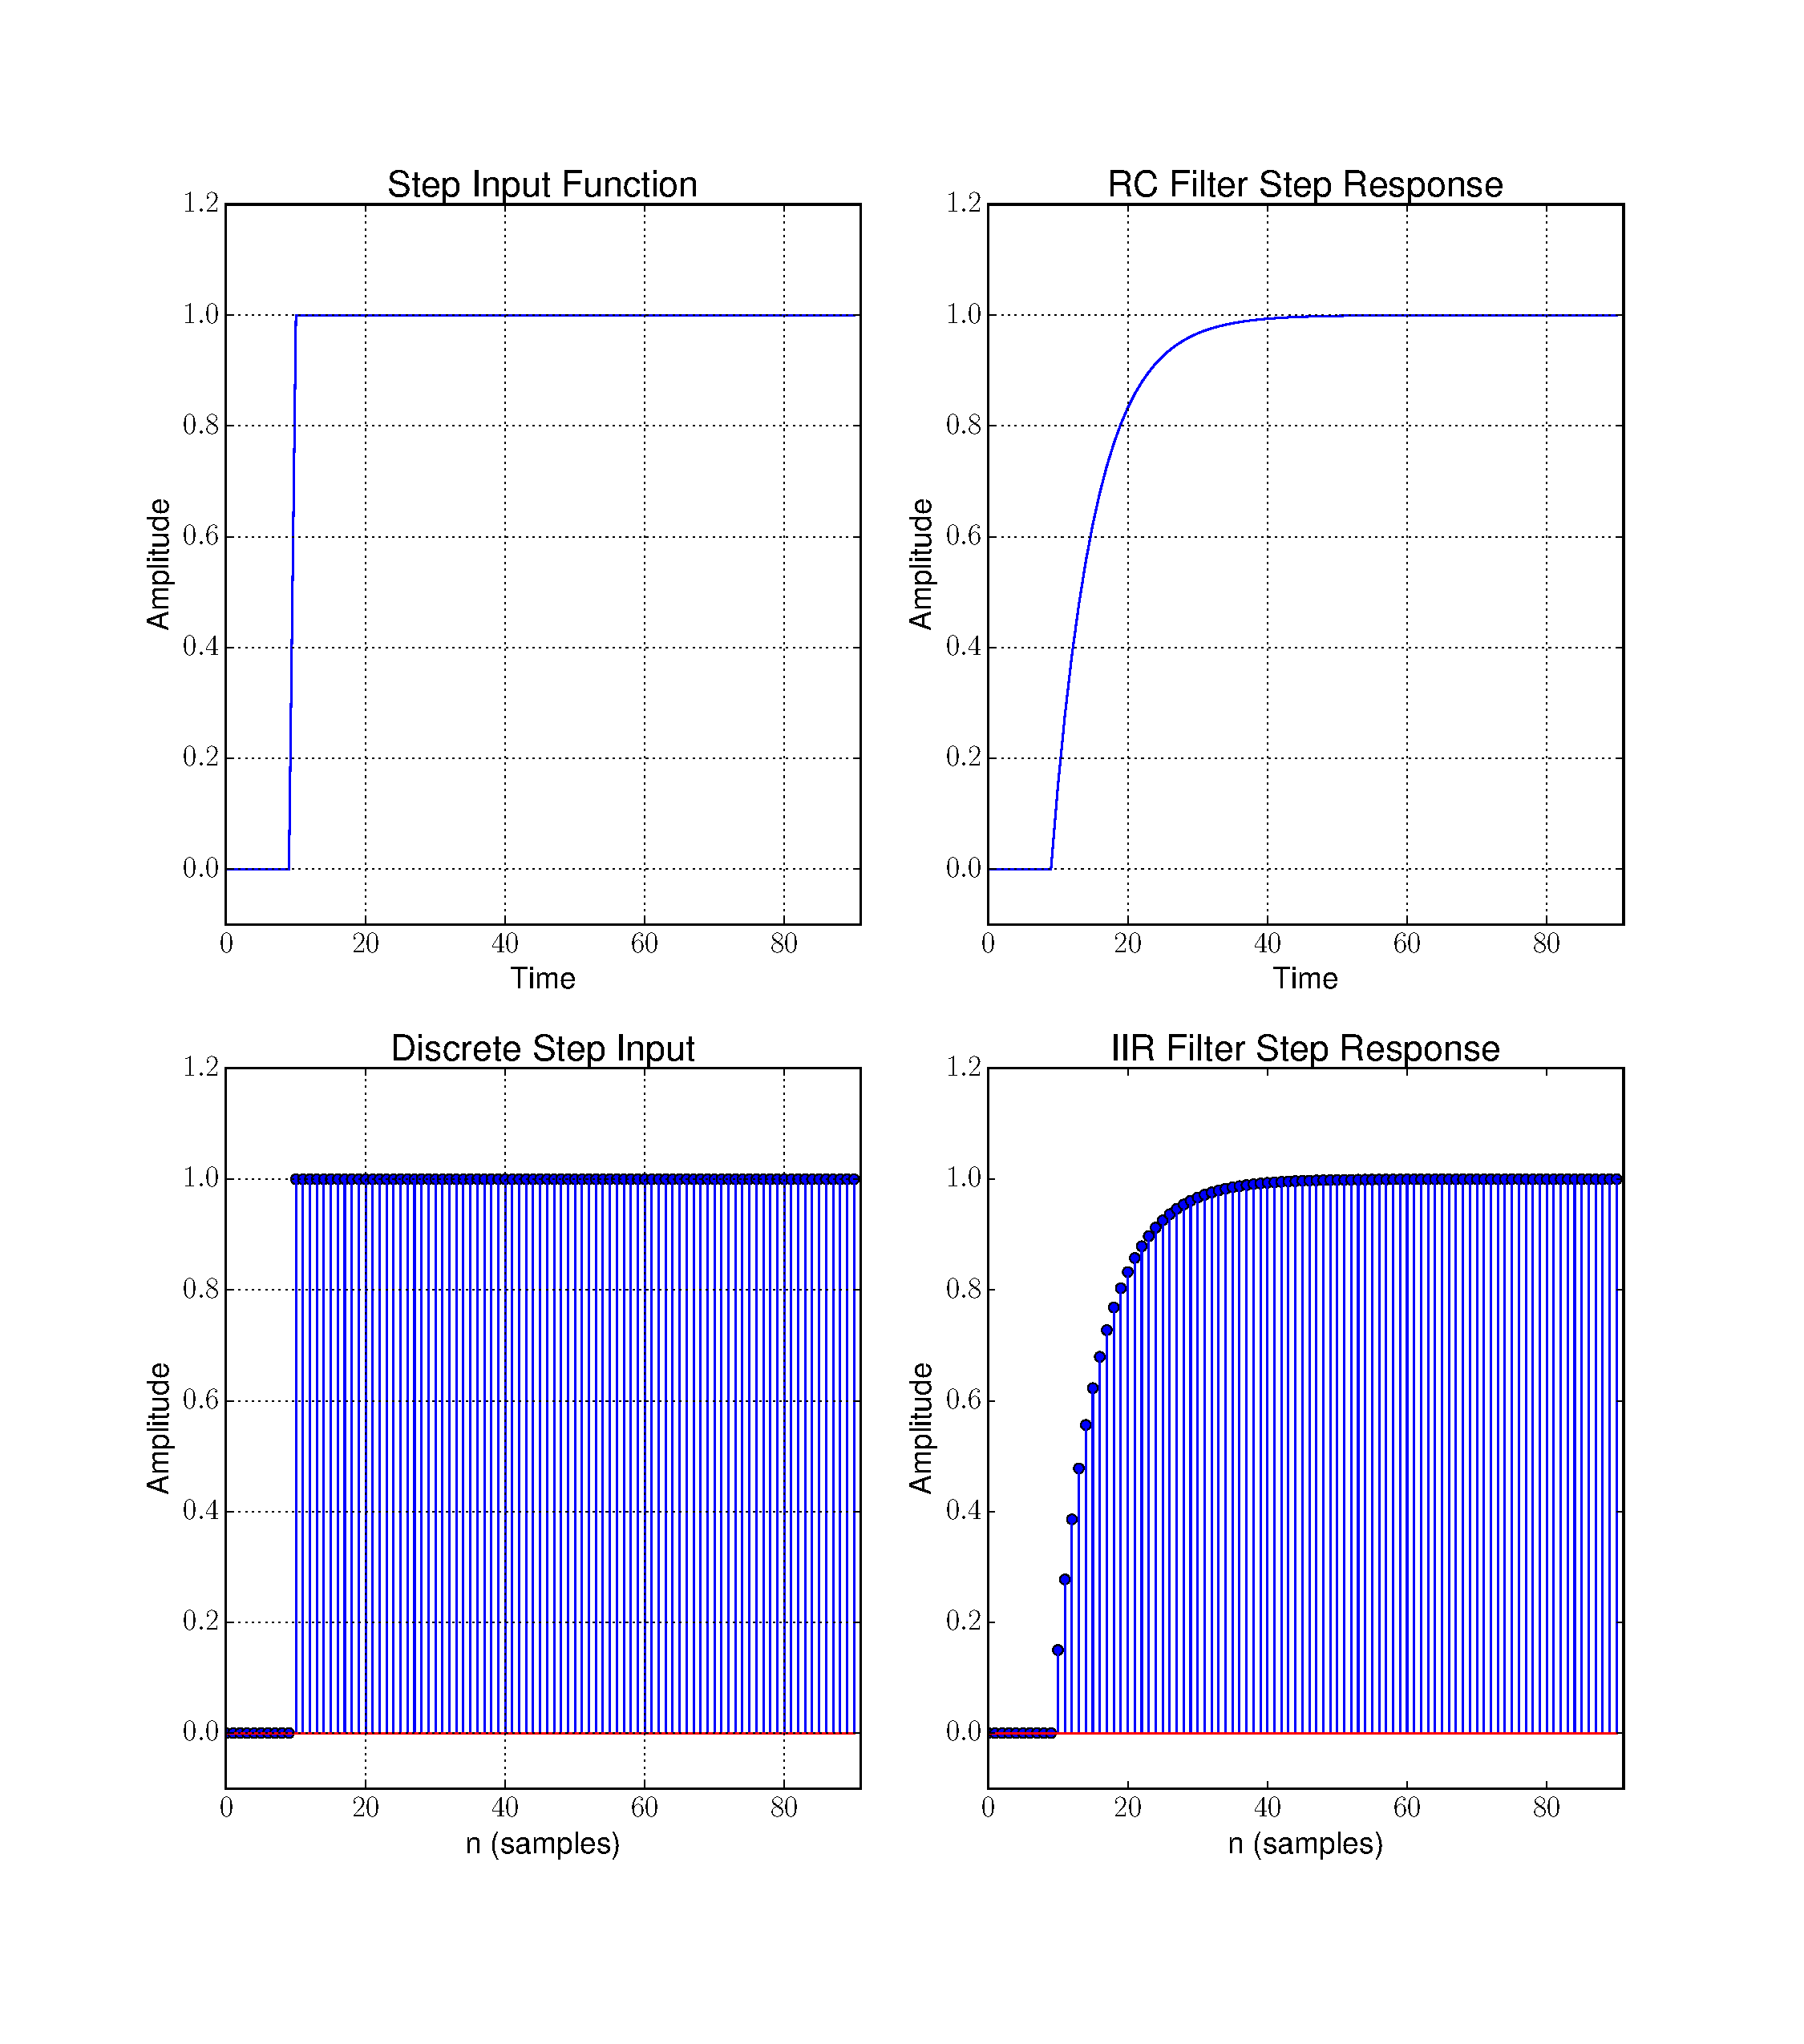
\includegraphics[width=12.5cm]{Experiments/Exp6/all_four.pdf}
\isucaption{Impulse input and the response of a RC low pass filter}
\label{rc_response}
\end{figure}
}

A single pole IIR filter is also known as a recursive filter as the mathematical expression used to describe this filter is a recursive function shown in Equation \ref{iir_recursive}.  In Equation \ref{iir_recursive}, our discrete output ($y[n]$) is defined as the input signal ($x[n]$) and is added to the previous sample calculated.  The coefficients, $a_0$ and $b_1$ then define the impulse response of the filter.  Figure \ref{rc_response} shows the discrete step input given to the system and the output response.  This response is calculated using Equation \ref{iir_recursive}.

\begin{equation}\label{iir_recursive}
y[n] = a_0 * x[n] + b_1 * y[n-1]
\end{equation}

The coefficients $a_0$ and $b_1$ are determined in Equation \ref{iir_coefficients} for a low pass filter.  Here $x$ is the amount of decay between each sample and is also defined as between zero and one.  The higher value that $x$ is, the slower the decay between samples.  

\begin{equation}\label{iir_coefficients}
a_0 = 1 - x
b_1 = x
for
0 < x < 1
\end{equation}

An analog RC filter has a similar decay that is determined by multiplying the physical value of the resistor and capacitor used in the circuit shown in Figure \ref{rc_circuit}.  This value is the number of seconds it takes for the circuit to decay to 36.8\% of its final value.  Equation relates this time constant to our value of $x$ for a desired cutoff frequency of $f_c$.  

\begin{equation}
x = e^{-2 \pi f_{c}}
\end{equation}
%{\begin{figure}[h!tb] 
%\centering
%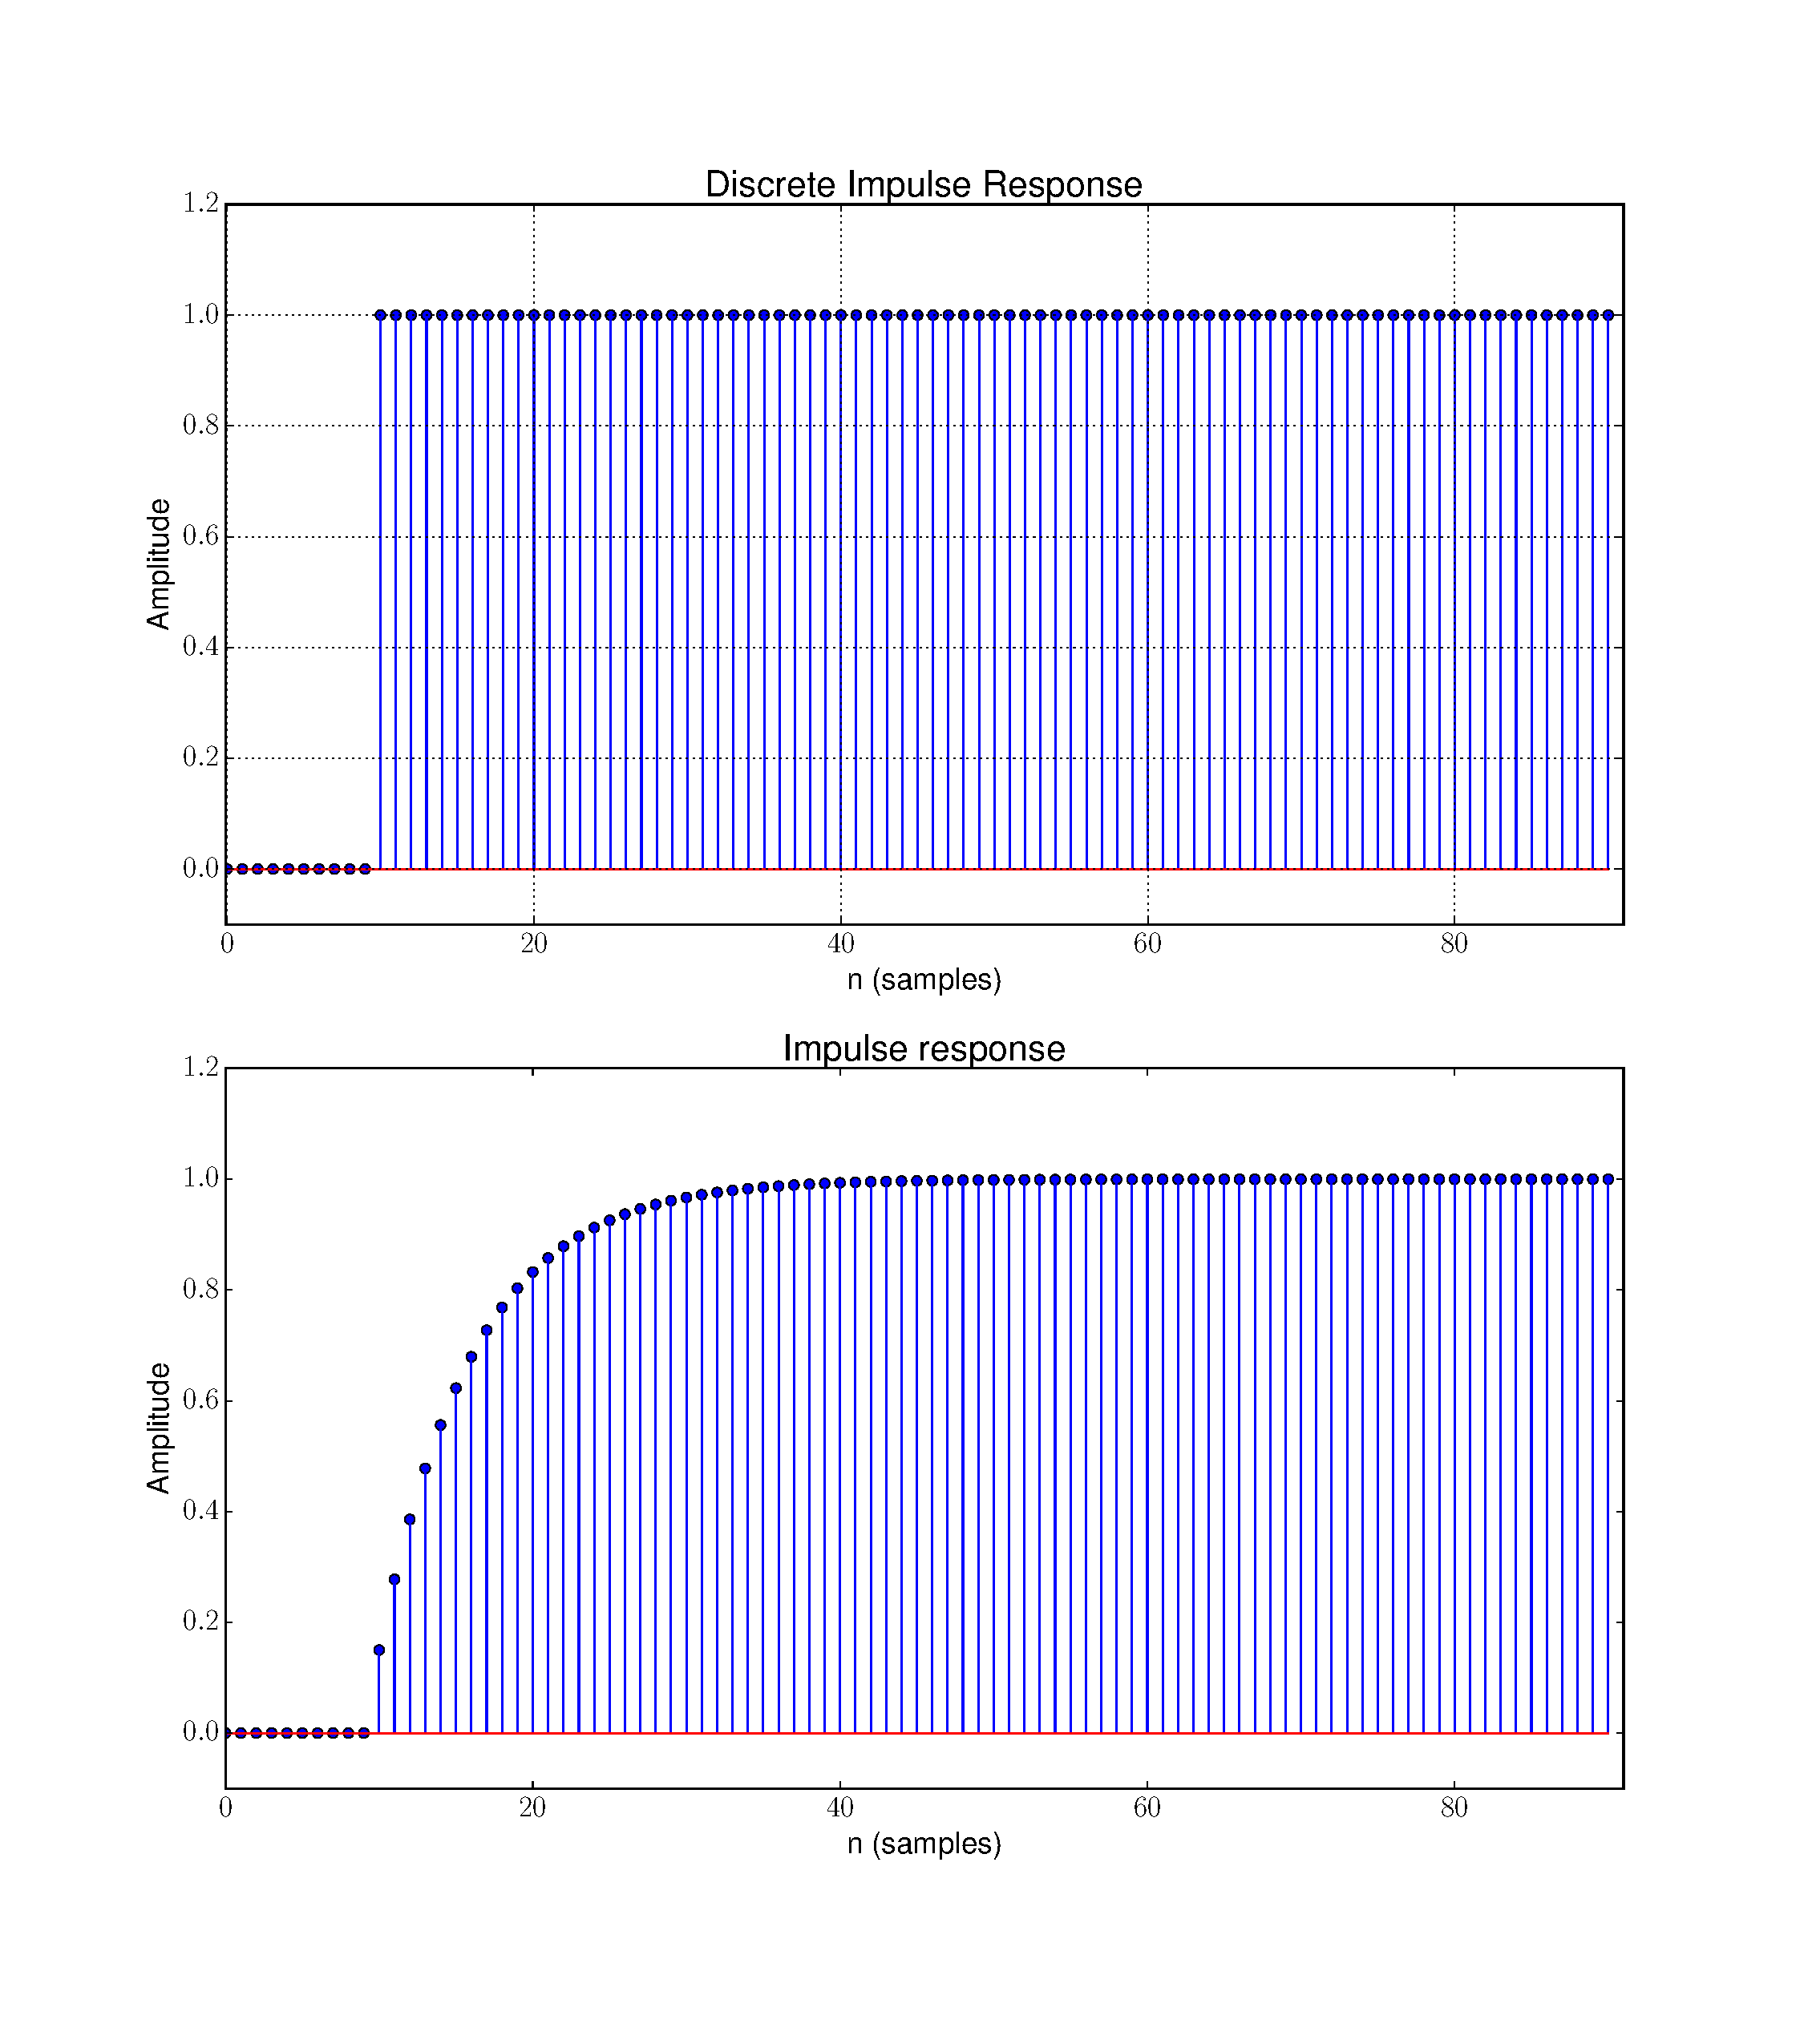
\includegraphics[width=17cm]{Experiments/Exp6/iir_response.pdf}
%\isucaption{Impulse input and the response of a RC low pass filter}
%\label{iir_response}
%\end{figure}
%}

It can be seen in Figure \ref{rc_response} that both the RC filter and the IIR filter respond identically to the same input, in this case a step function.  Therefore our single pole IIR filter functions identically to a RC low pass filter.  

%Re-added stuff on IIR filters per Phillips request

In Figure \ref{rc_circuit}, the input is $V_{in}$, the resistance value is $R$, the capacitance value is $C$ and the output is $V_{out}$.  This circuit can be represented by Equation \ref{eq:rc_circuit_eq}.

\begin{equation}\label{eq:rc_circuit_eq}
\frac{V_{in}-V_{out}}{R}=C\frac{dV_{out}}{dt}
\end{equation}

Equation \ref{eq:rc_circuit_eq} represents the differential equation relating the input voltage $V_{in}$ to the output voltage $V_{out}$.  We can substitute the input to the RC circuit ($V_{in}$) as the input to Equation \ref{IIR_eq} or $x_n$.  The output of our RC circuit ($V{out}$) can also be expressed as the output in Equation \ref{IIR_eq} which is $y_n$.  However, in order to do that we must move from the continuous domain to the discrete domain that our digital filter operates in.  This is done by showing the relationship between our sampling frequency $f_s$ and our period or time between samples, $T$ and is shown in Equation \ref{sampling_rate_eq}.

\begin{equation}\label{sampling_rate_eq}
T=Time Between Samples=\frac{1}{f_s}
\end{equation}

Next we rewrite our difference equation by substituting $x_n$ and $y_n$ into Equation \ref{eq:rc_circuit_eq} which results in an approximated finite difference equation shown in Equation \ref{diff_xn_yn}.

\begin{equation}\label{diff_xn_yn}
\frac{x_n-y_n}{R}=C\frac{y_n-y_{n-1}}{T}
\end{equation}

We can now solve for $y_n$ algebraically and this results in our final Equation \ref{final_IIR_RC}.

\begin{equation}\label{final_IIR_RC}
y_n=\frac{T}{T+RC}x_n+\frac{RC}{T+RC}y_{n-1}
\end{equation}

Equation \ref{final_IIR_RC} shows an IIR filter that has a frequency response that closely approximates an RC circuit.  The approximation improves as $T$ approaches zero or our sampling rate approaches infinity.

To design the filter we need to look at what our desired cut-off frequency needs to be.  For a RC filter, our resistance and capacitance define our cutoff frequency ($f_c$) and has the relationship shown in Equation \ref{fc_RC}.

\begin{equation}\label{fc_RC}
f_c=\frac{\sqrt{3}}{2\pi RC}
\end{equation}

Given our desired cutoff frequency we can determine our combined $RC$ value by rearranging Equation \ref{fc_RC} algebraically to Equation \ref{RC_fc}.

\begin{equation}\label{RC_fc}
RC=\frac{\sqrt{3}}{2\pi f_c}
\end{equation}

The $RC$ values are also referred to as the time constant of the circuit and we do not need to find the individual R and C values.  An example of how we can find the coefficients of our IIR filter, given a desired cutoff frequency of $f_c$ is shown next.  

For a low pass filter, we want a cutoff frequency ($f_c$) of 1000 Hz.  Given this and using Equation \ref{RC_fc} we can determine our time constant to be 2.757 x $10^-4$ or 275.7 microseconds.  If our sample rate is 1 MHz, then our $T$ value is 1 x $10^-6$ or 1 microsecond.  Plugging these values into Equation \ref{final_IIR_RC} results in the coefficient $c_0 = 0.0036$ and $d_1=0.9964$.

%------------------------------------------------------


GNURadio includes a program that allows us to define our filter and it will generate the coefficients and taps needed for our filters.  Chapter \ref{ch:exp_design} goes into more depth on this program.

\subsection{Bandwidth limiting and filtering}

\emph{Bandwidth limiting.}  Bandwidth limiting is the process of defining the frequency band over which a radiometer measures power.  For a traditional radiometer, this is typically accomplished using analog filters.  Within a SDR-based radiometer, bandwidth is controlled by the sampling rate of the Analog to Digital Converter (ADC).  However, in the N200 SDR used in this thesis, the ADC clock is fixed at 100 MHz.  Therefore the FPGA decimates the data to reduce the bandwidth from the ADC, but only by integer values of the divisor.

\emph{Filtering.}  There are instances when the frequency being observed requires additional filtering (i.e. RFI mitigation, see section \ref{Exp3_results}).  Traditional radiometers deploy analog band-pass or band-reject filters to accomplish this, while in this thesis we show similar functionality can be obtained by implementing software defined filters.

\section{Software Defined Radio Based Radiometer Control System}

A traditional radiometer will be designed with fixed parameters such as bandwidth and integration time.  While changes can be made, it requires changes to the radiometer's physical hardware.  A SDR-based radiometer allows us to control several functions that defines how it operates as a radiometer.  These changes can be made while the radiometer is operating since these operations happen in the digital domain and is defined by software. The following items are controlled by software in our SDR-based radiometer: 1) Center frequency, 2) Bandwidth ($\beta$), 3) Integration time ($\tau$), and 4) Gain.

The GUI for the SDR-based radiometer was designed knowing that these parameters such as frequency, bandwidth and integration time can be changed.  Because these controls impact both the performance of the radiometer and in what frequency range the radiometer operates in, it was important to have these controls clearly marked.  Figure \ref{radiometer_gui} shows a screen-shot of the GUI.

{\begin{figure}[h!tb] 
\centering
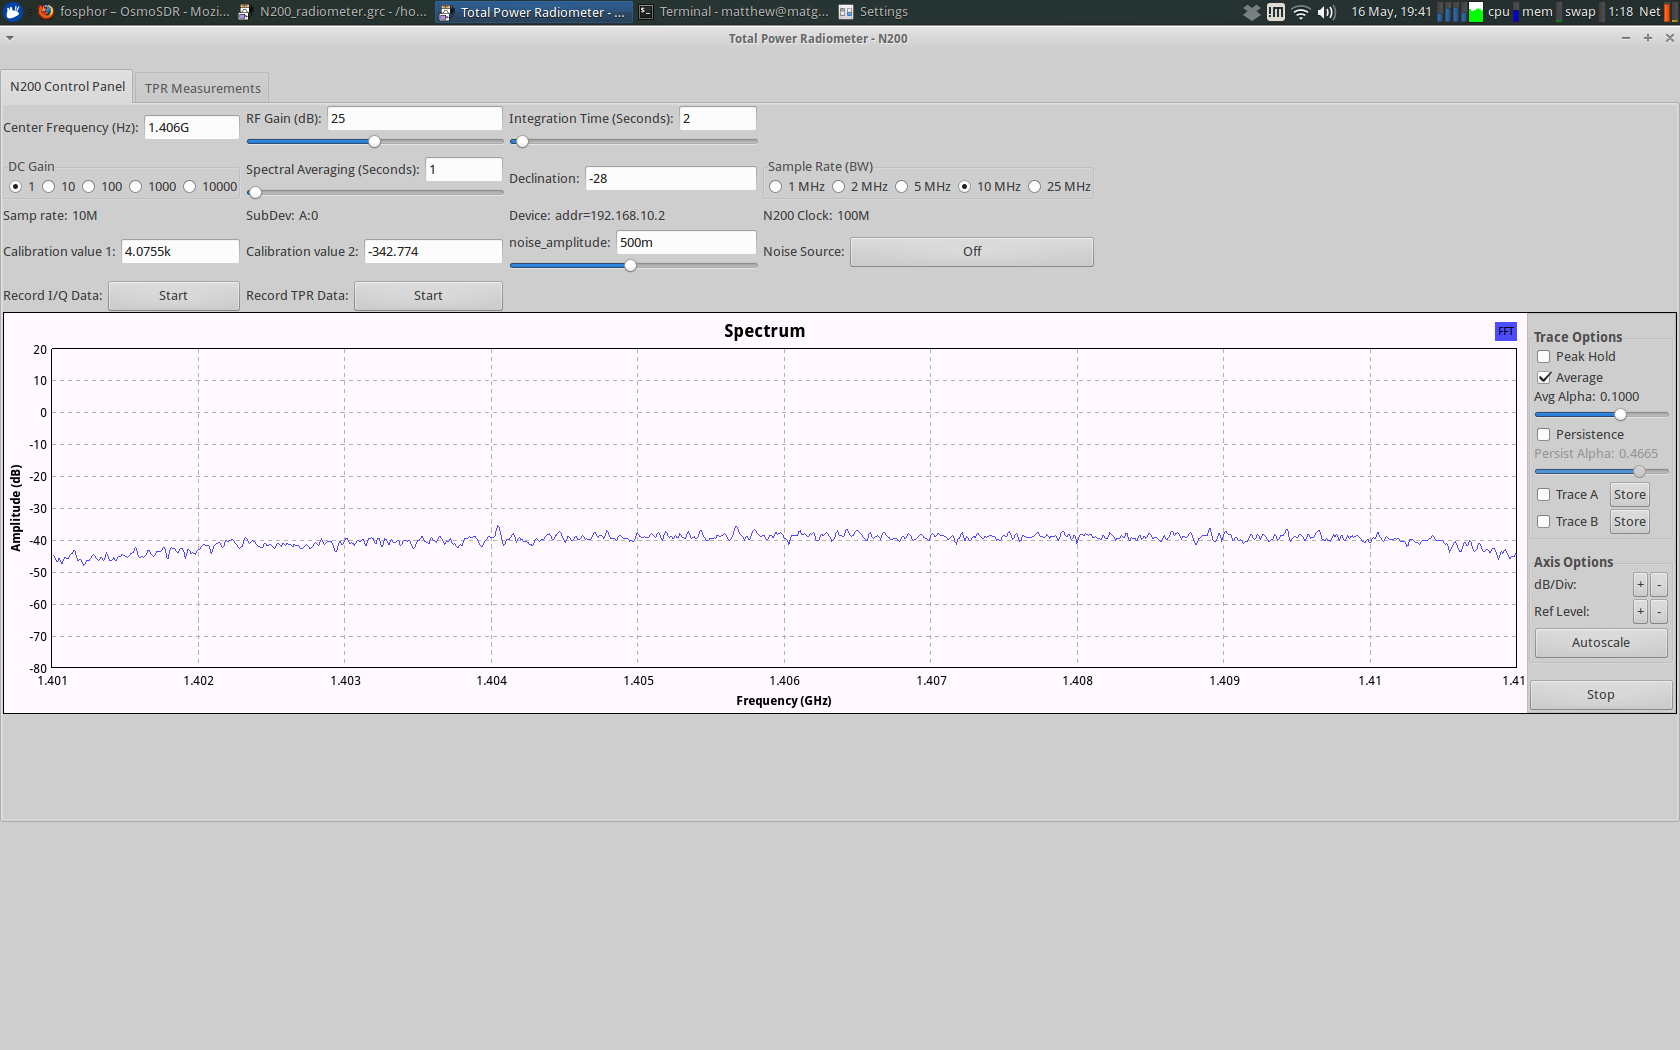
\includegraphics[width=16cm]{Images/radiometer_gui.png}
\isucaption{A screenshot of the interface made for communication with and controlling the software defined radio}
\label{radiometer_gui}
\end{figure}
}

The bandwidth, $\beta$, and our integration time, $\tau$, both impact our sensitivity or $NE\Delta T$ of the radiometer as defined in Equation \ref{NEAT_EQ}.  The bandwidth can be changed by changing the sample rate of the SDR.  The sample rate effectively controls the bandwidth in which the SDR is operating at.  This also gives us a band-pass filter as well, since the SDR will not respond to frequencies outside of this bandwidth.  The integration time parameter is set by the user through the GUI and allows us to change the integration time in seconds.  This directly controls the time constant for the IIR filter used to smooth the data.

The SDR-based radiometer in this thesis uses Low Noise Amplifiers (LNAs) to increase the gain of the system.  The DBSRX2 hardware, described in Section \ref{N200_HW}, also has Programmable Gain Amplifier (PGA) that is controlled by software.  This allows for additional gain to be added or removed as needed.  Next we will also look at how the data is displayed and stored in the software defined radiometer.

\section{SDR-based radiometer data display}

The information from the software defined radio can be displayed through GNURadio to show relevant information to the user.  Currently, our SDR-based radiometer can display spectrum information and total power information.  Spectrum information is used to verify the signal is clean and free of interference. Total power information is displayed as both un-calibrated values and calibrated values, assuming the correct calibration terms have been provided.  This includes a display in a "ticker tape" graph and as a bar graph.  Figure \ref{radiometer_tpr_display} shows a screen-shot of the total power display.  

{\begin{figure}[h!tb] 
\centering
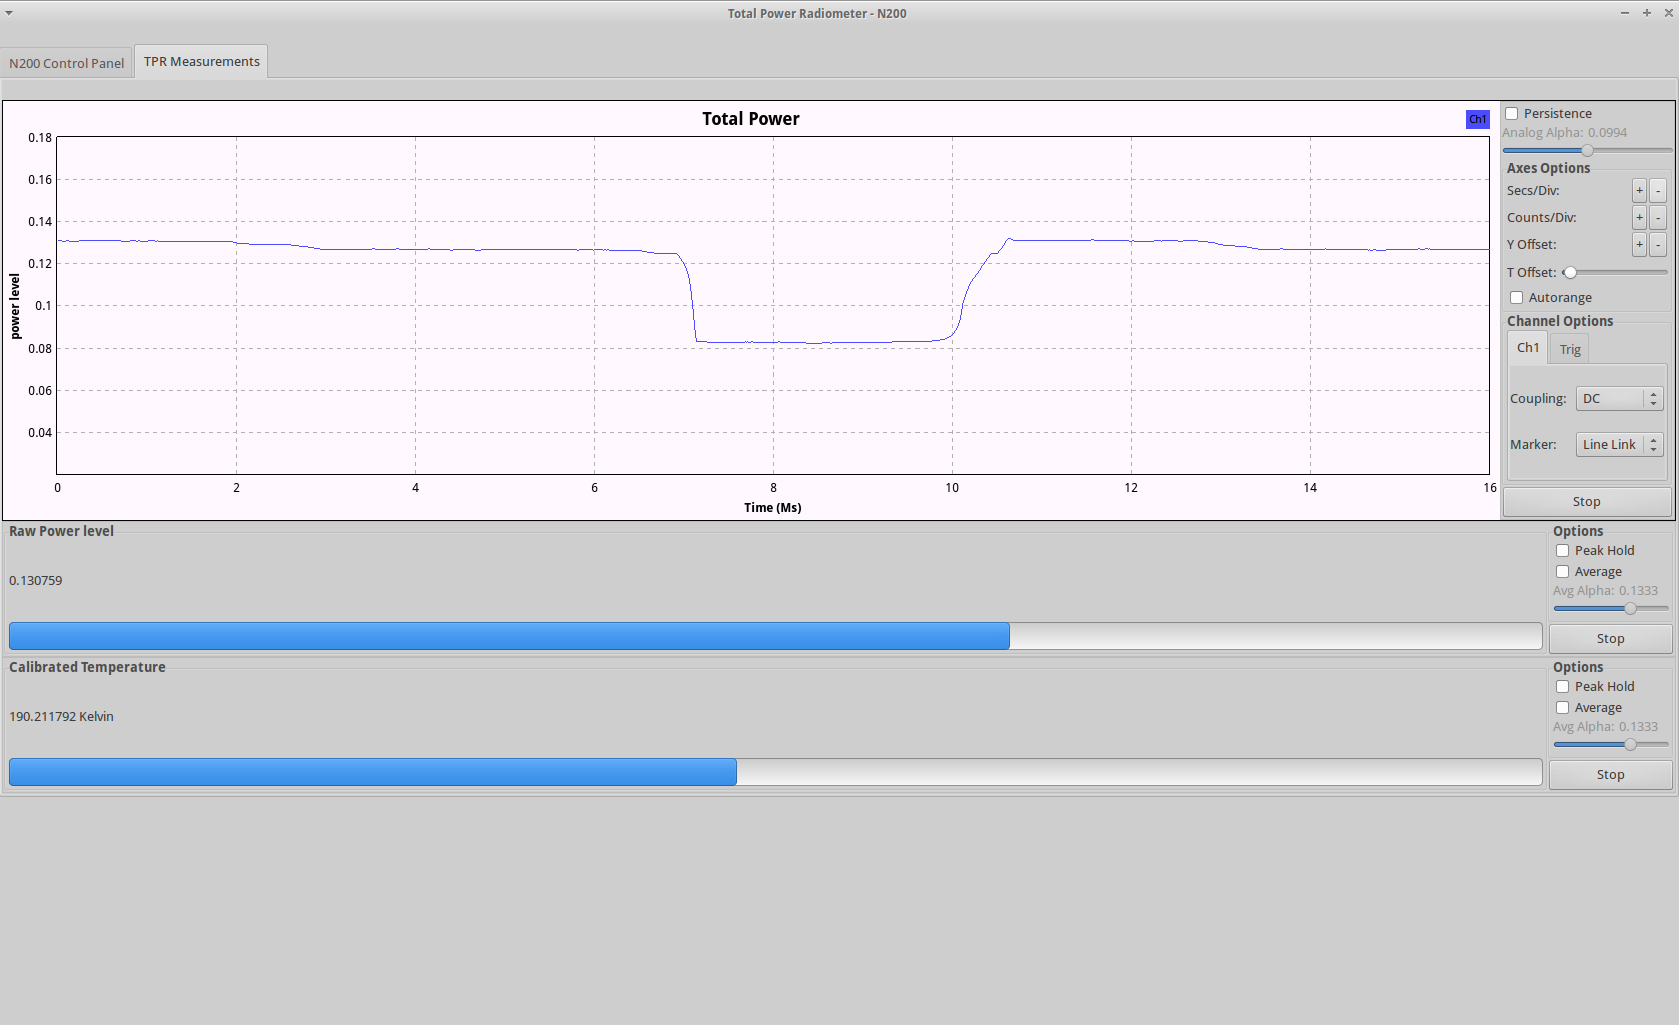
\includegraphics[width=16cm]{Images/Lab1_TPR_at_end_exp.png}
\isucaption{A screenshot showing the ticker tape display for the total power readings.  In addition, raw and calibrated noise temperature is shown below.}
\label{radiometer_tpr_display}
\end{figure}
}

%----------------------------------------------------------------------------------
%Everything below this needs to be moved/shifted or deleted

